\section{Question 2: Rheology}

The different DS values for the differennt batches are cacultad as

\begin{equation}
    DS = \frac{n_{\text{methacrylamide}}}{n_{\text{amine}}},
    \label{eq:DS}
\end{equation}

in which $n_{\text{amine}} = 0.385\unit{mmol}$ and

\begin{equation}
    n_{\text{methacrylamide}} = \frac{I(5.5\unit{ppm})+I(5.75\unit{ppm})}{2\cdot k},
    \label{eq:nMA}
\end{equation}

where $k$ is calculated as

\begin{equation}
    k = \frac{I(1\unit{ppm})}{6\cdot n_{\text{VLI}}},
    \label{eq:j}
\end{equation}

with $n_{\text{VLI}}=0.64\unit{mmol}$. All the data, from the NMR spectra on UFORA, and the cacultad values are found in table \ref{tab:researcher1}.

\begin{table}[H]
    \centering
    \begin{tabular}{ccccccc}
      batch & $I(1\unit{ppm})$ & $I(5.5\unit{ppm})$ & $I(5.75\unit{ppm})$ & $k$ [1/mmol]& $n_{\text{methacrylamide}}$ [mmol] & DS [\%]\\
      \hline
      A & 142871.9 & 4918.98 & 4790.75 & 37206.22 & 0.130 & 34\\
      B & 166032.1 & 12362.5 & 12140.48 & 43237.53 & 0.283 & 74\\
      C & 114480.1 & 10858.83 & 1162.68 & 29812.83 & 0.369 & 96\\
    \end{tabular}
    \caption{DS values for the differennt batches}
    \label{tab:researcher1}
\end{table}

\begin{figure}[H]
    \centering
    \begin{subfigure}[b]{0.45\textwidth}
    \centering
    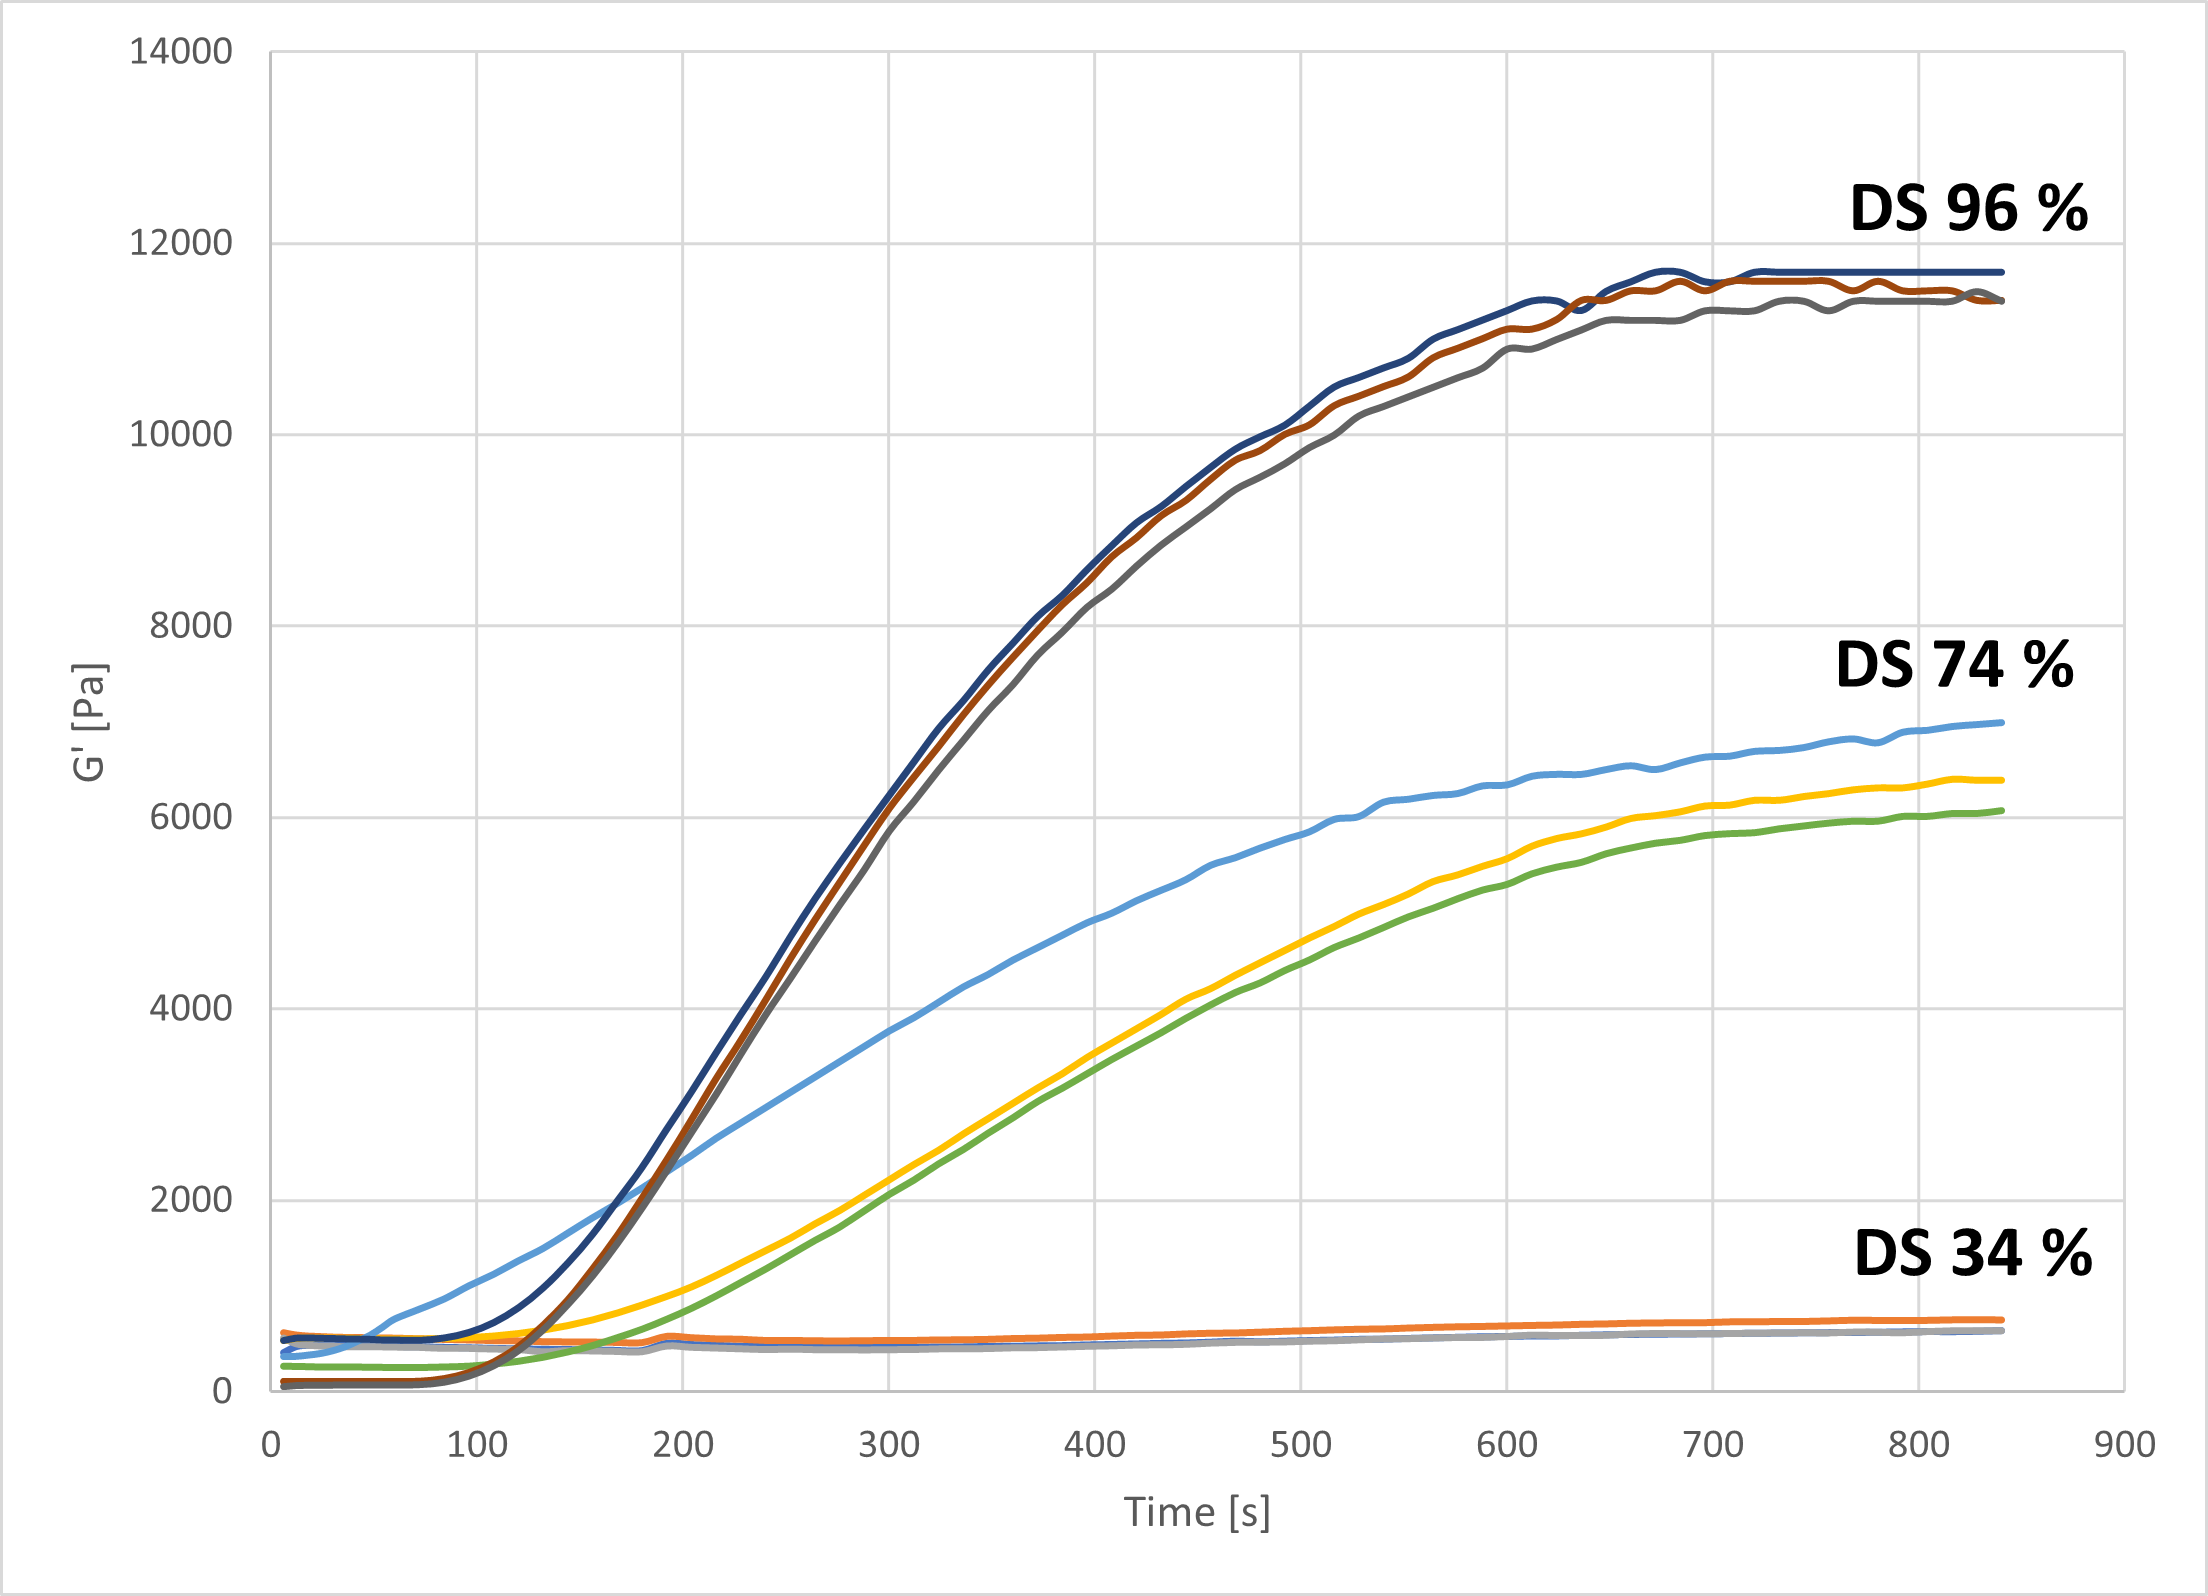
\includegraphics[width=\textwidth]{in_situ_UV_crosslinking_person1.png}
    \end{subfigure}
    \begin{subfigure}[b]{0.45\textwidth}
    \centering
    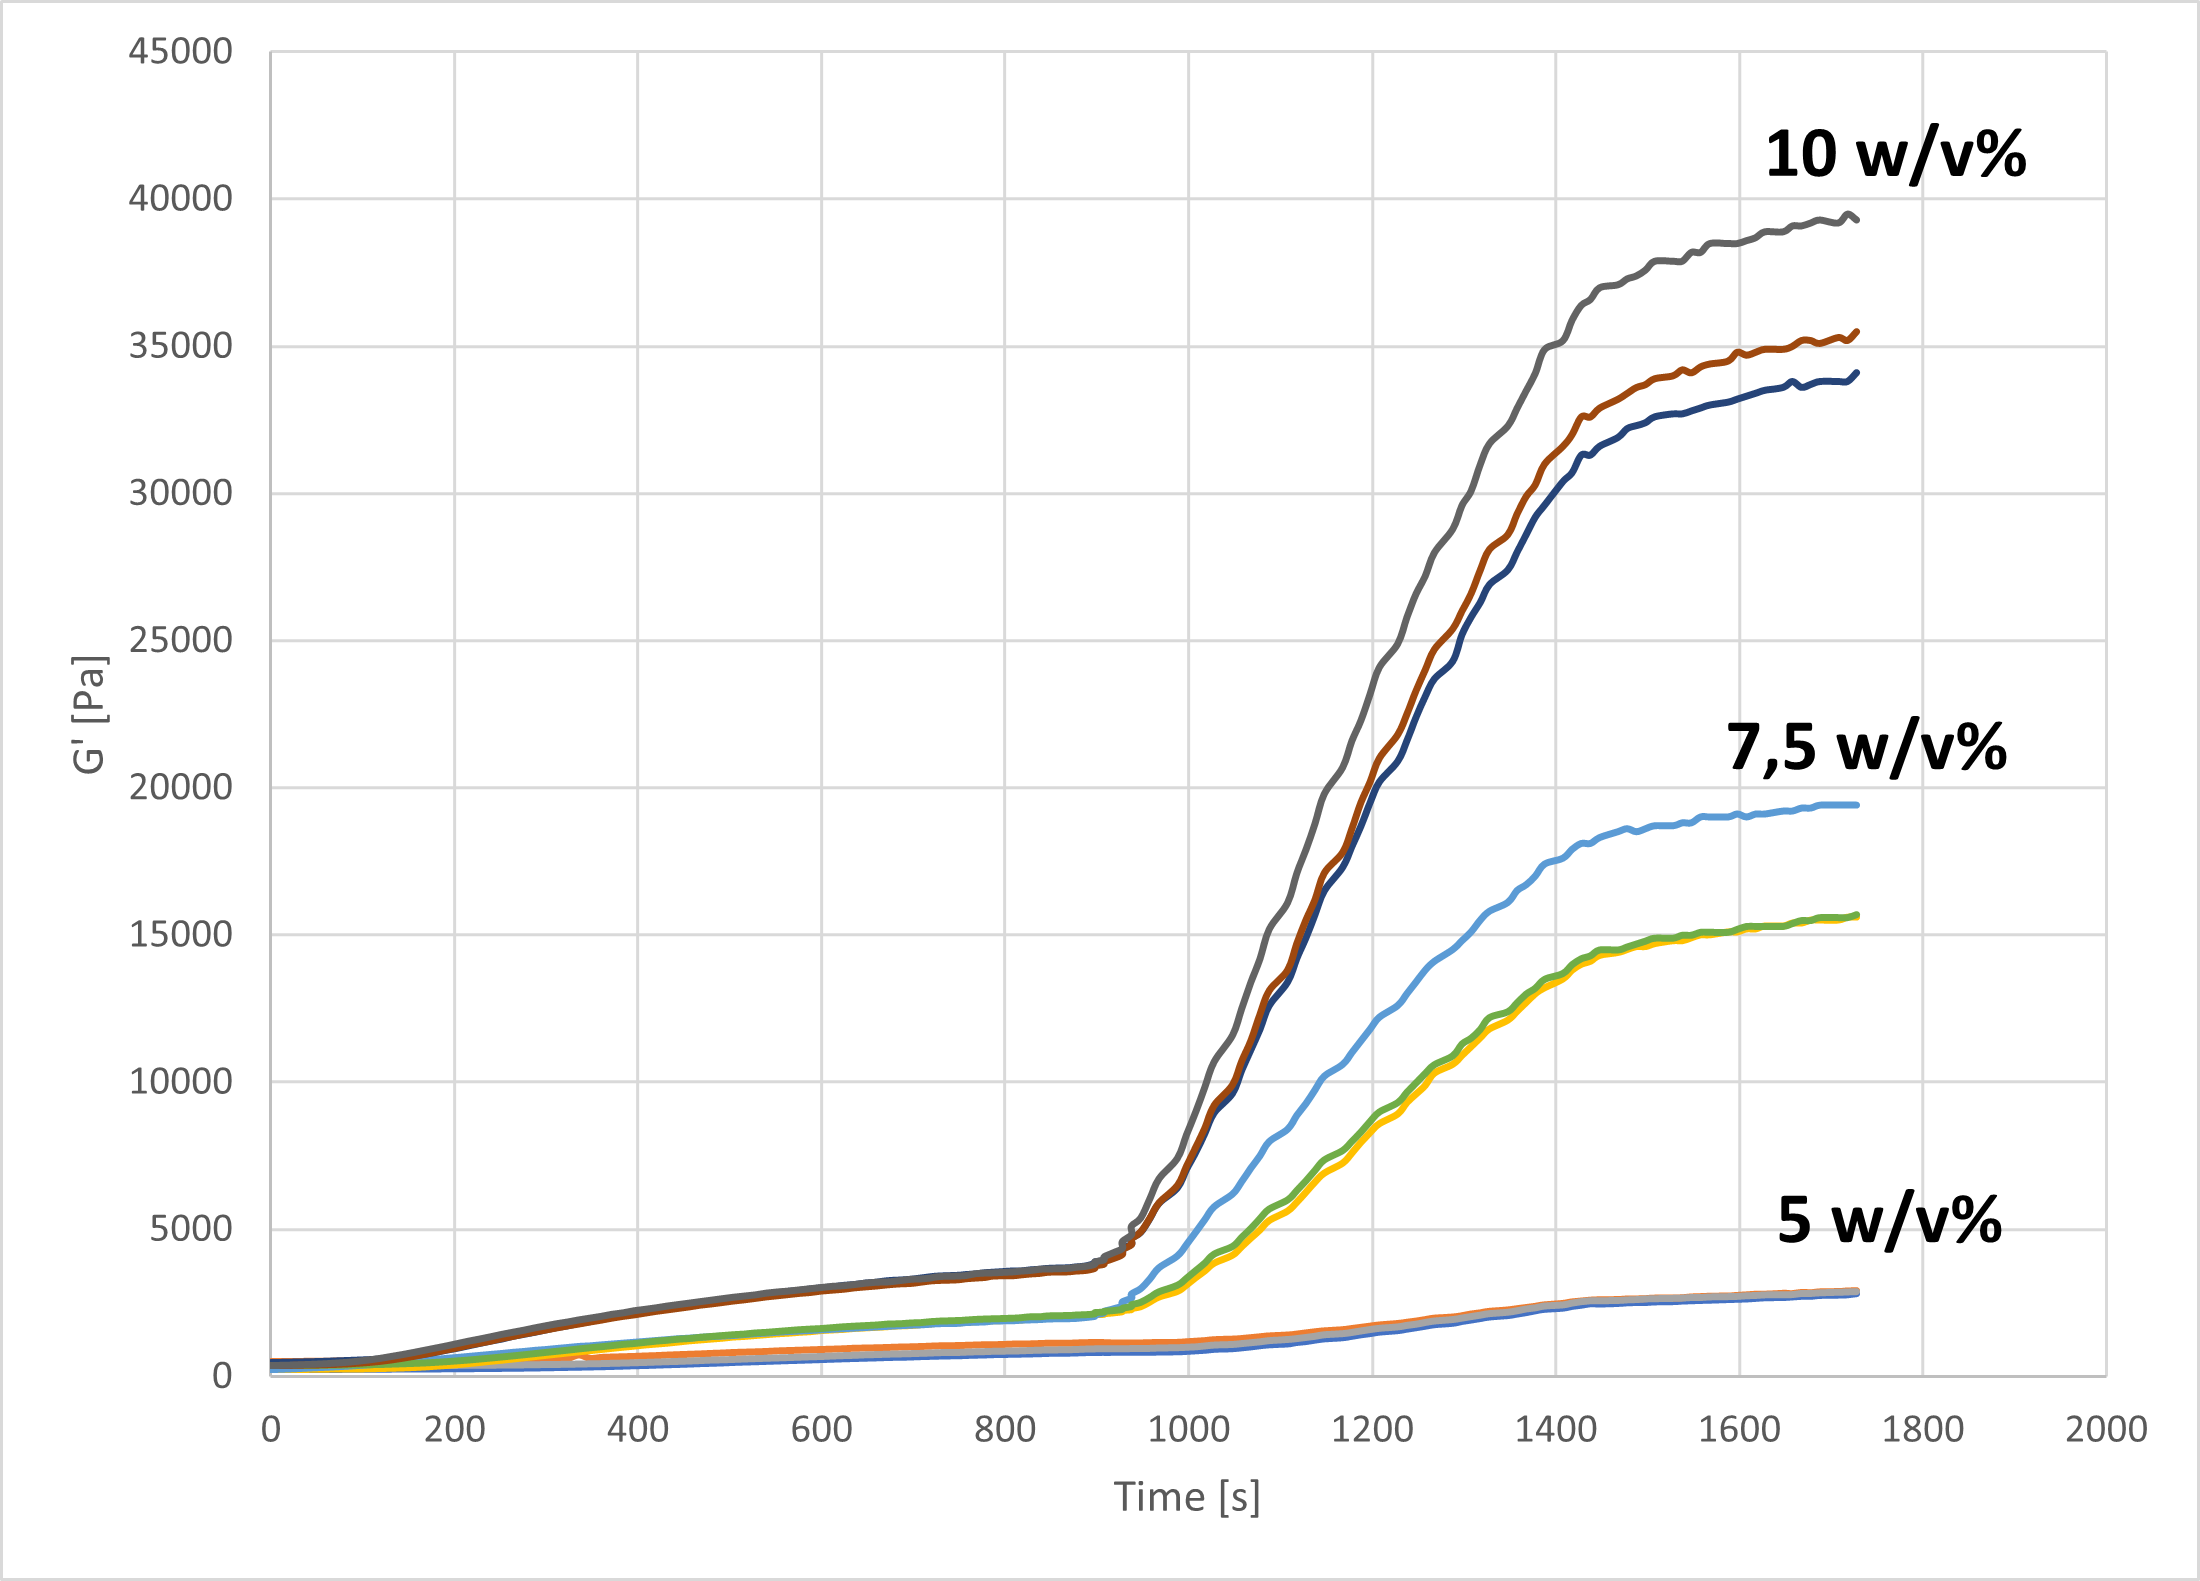
\includegraphics[width=\textwidth]{in_situ_UV_crosslinking_person2.png}
    \end{subfigure}
    \caption{Rheological in-situ UV-crosslinking with varying DS (right) and varying w/v\% (left)}
    \label{fig:rheo}
\end{figure}

In figure \ref{fig:rheo} the rheological data from the different researchers is displayed. The storage modulus $G'$ increases for increasing DS as well as for increasing w/v\%. 
$G'$ is a parameter that relates to the elasticity of the obtained material, it is the amount of energy stored in the material due to deformation. High $G'$ values indicate that the material is stiff and lower values indicate a more elastic behavior. 
In this rheology setup, gelMA is subjected to an oscillating stess or strain while irradiated by UV light. The gelMA is crosslinking due to the UV-ligth and $G'$ is measured during this crosslinking proces. More crosslinks imply a stronger force holding the material structure 
together. More crosslinks can be induced by higher DS values or higher concentration of gelMA. This theory corresponds perfeclty with the obtained data. Furthermore a steaper increase of $G'$ indicates a higher crosslinking speed. After most gelMA is crosslinked $G'$ 
comes to a plateau value.

A difference between the two measurements can be observed. The data from the left graph (researcher 1) is collected over a smaller time interval and the maximal "$G'$ is much lower compaired to that of researcher 2. This comparison can be made since both researchers have used batch C at 10 w/v\%. 
One possibility that causes this difference in measurement is the amount of photo-initiator added to the gelMA. 

